\section{Experiments}
\label{sec:experiments}

To demonstrate the effectiveness of GAF in practice, we train ResNet image classifiers on the CIFAR-100 and CIFAR-100N-Fine datasets using distributed data-parallelism comparing both baseline averaging-based gradient aggregation and GAF-based gradient aggregation. 

\begin{table*}[ht!]
\centering
% \resizebox{\textwidth}{!}{%
\begin{tabular}{@{}lcccccccccc@{}}
\toprule
Dataset & \multicolumn{9}{c}{CIFAR-100} & CIFAR-100N-Fine \\
\midrule
Label Error & 0\% & 5\% & 15\% & 20\% & 30\% & 40\% & 50\% & 60\% & 75\% &  \\
\midrule
GAF & 63\% & 61\% & 60\% & 58\% & 54\% & 53\% & 48\% & 39\% & 13\% & 61.4\%  \\
Averaging & 62\% & 58\% & 53\% & 50\% & 40\% & 38\% & 33\% & 20\% & 11\% & 52.1\% \\
\bottomrule
Improvement & +0.2\% & +3\% & +7\% & +8\% & +14\% & +15\% & +15\% & +19\% & +2\% & +9.3\% \\
\bottomrule
\end{tabular}%
% }
\caption{Image classification validation accuracy of ResNet18 on CIFAR-100 and CIFAR-100N-Fine when trained with GAF-based vs. averaging of micro-gradients. Improvement is the absolute increase in validation accuracy of GAF-based training over the baseline averaging.}
\end{table*}

\subsection{CIFAR-100}

We train RestNet18 on two A40 GPUs on the CIFAR-100 dataset using SGD with momentum and and reduction of the learning rate (learning rate) on validation plateaus with schedule patience of 100 and 0.1 discount. We use an initial learning rate of 0.01. We also applied L2 regularization with a weight decay of 0.01. In all cases, unless otherwise specified, we use a macrobatch of size $m = 200$ with $u = 100$ images per microbatch (exactly 1 sample per class) to ensure each microbatch has the same distribution of data over the training set. We flip each label with a random other classes label for x\% of the labels, for $ x \in \{0,5,15,30,40,50,60,75,80,90\}$, and maintain those incorrect label for the entirety of that run's training (i.e. symmetric noise). For each experiment we found the optimal value of the cosine distance threshold hyperparameter $\tau$ by performing a grid search of values from 0.95 to 1.05 with a step of 0.02 across different batch sizes. We compare with a baseline-training of ResNet18 where the cosine distance threshold is set to 2, which admits all gradients and is equivalent to averaging training weights when $k = 2$. We run for 500k iters for all runs, and observe convergence around 270k iterations for baseline and GAF runs. 

For the no error case, we observe cosine distance threshold of 1 yields best performance. Once errors are introduced we observe a cosine distance of 0.97 provides the best performance. 

As shown in \Cref{fig:cifar100_over_noise_results}, we see a 0.2\% improvement over baseline without added noise to the CIFAR-100 dataset. As we add more and more noise to the labels, the GAF-trained models show increasing improvement over baseline until 60\% where it beats baseline model by 18.4\% when $\tau = 0.97$.

\begin{figure}[t]
    \centering
    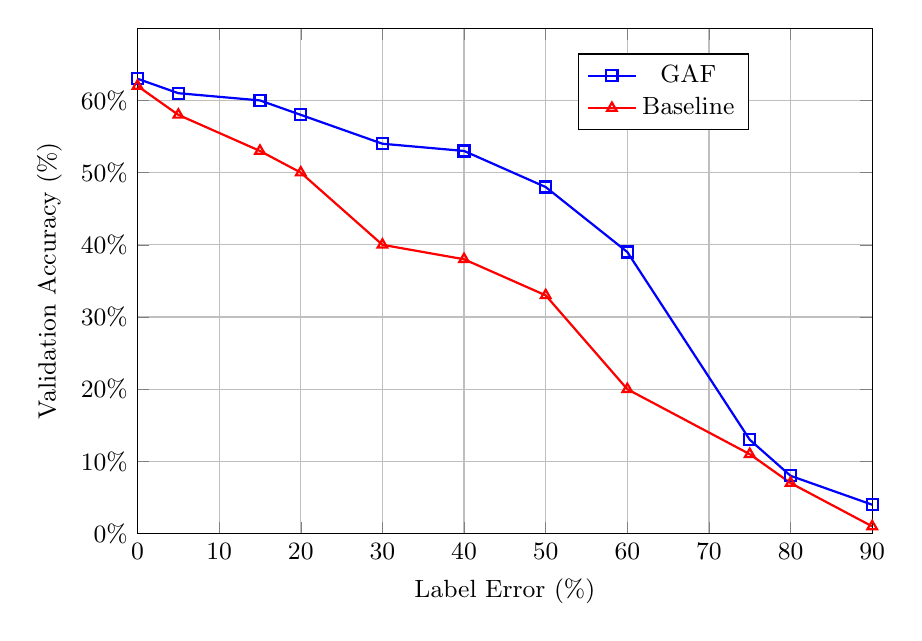
\begin{tikzpicture}
        \begin{axis}[
            width=0.9\linewidth,
            height=8cm,
            xlabel={Label Error (\%)},
            ylabel={Validation Accuracy (\%)},
            xmin=0, xmax=90,
            ymin=0, ymax=70,
            xtick={0, 10, 20, 30, 40, 50, 60, 70, 80, 90},
            ytick={0, 10, 20, 30, 40, 50, 60},
            yticklabel={\pgfmathprintnumber{\tick}\%},
            legend style={font=\small, at={(0.6, 0.95)}, anchor=north west},
            grid=major,
            % title={CIFAR-100 Validation Accuracy of GAF over Baseline},
            label style={font=\small},
            tick label style={font=\small}
        ]

        % Plot for Validation Accuracy - GAF
        \addplot[
            color=blue,
            mark=square,
            thick
        ] coordinates {
            (0, 63) (5, 61) (15, 60) (20, 58) (30, 54) (40, 53) (50, 48) (60, 39) (75, 13) (80, 8) (90, 4)
        };
        \addlegendentry{GAF}

        % Plot for Validation Accuracy - Baseline
        \addplot[
            color=red,
            mark=triangle,
            thick
        ] coordinates {
            (0, 62) (5, 58) (15, 53) (20, 50) (30, 40) (40, 38) (50, 33) (60, 20) (75, 11) (80, 7) (90, 1)
        };
        \addlegendentry{Baseline}

        \end{axis}
    \end{tikzpicture}
    \caption{Validation accuracy on CIFAR-100 with symmetric noisy labels for ResNet18 trained with and without GAF.}
    \label{fig:cifar100_over_noise_results}
\end{figure}

Additionally, we see in \Cref{fig:cifar100_validation_over_cosine_distance} that the performance improvement from GAF-based training ultimately decreases as we increase our cosine distance threshold. As we increase cosine distance threshold beyond 0.97, the improvement from GAF filtering goes away as the filter starts admitting more noise in our gradients, and removing the ability to discern good from bad micro-gradients.

\begin{figure}[ht!]
    \centering
    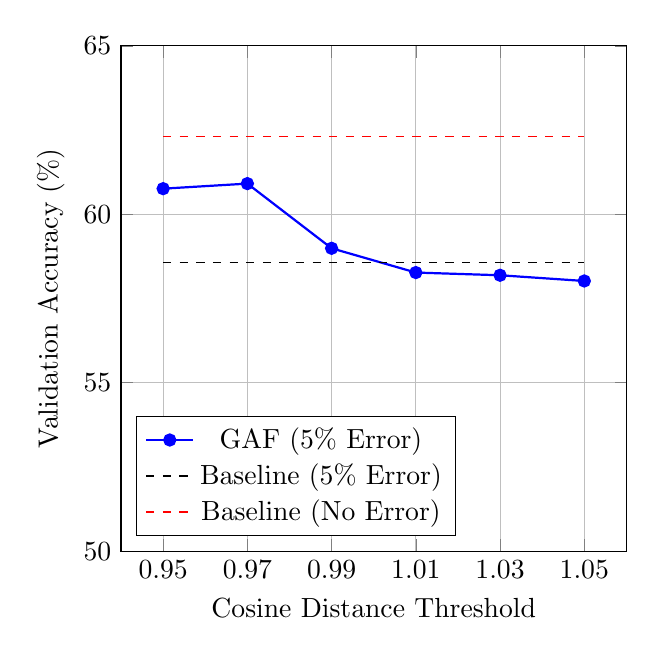
\begin{tikzpicture}
        \begin{axis}[
            % title={GAF over Cosine Distance},
            xlabel={Cosine Distance Threshold},
            ylabel={Validation Accuracy (\%)},
            xmin=0.94, xmax=1.06,
            ymin=50, ymax=65,
            xtick={0.95, 0.97, 0.99, 1.01, 1.03, 1.05},
            ytick={50, 55, 60, 65},
            legend pos=south west,
            grid=both,
            % width=\textwidth,
            width=8cm,
            height=8cm,
        ]

        % Plot validation accuracy
        \addplot[
            color=blue,
            mark=*,
            thick,
        ] coordinates {
            (0.95, 60.76)
            (0.97, 60.91)
            (0.99, 58.99)
            (1.01, 58.27)
            (1.03, 58.19)
            (1.05, 58.02)
        };
        \addlegendentry{GAF (5\% Error)}

        % Lower bound (baseline performance with error)
        \addplot[
            color=black,
            dashed,
        ] coordinates {
            (0.95, 58.57)
            (0.97, 58.57)
            (0.99, 58.57)
            (1.01, 58.57)
            (1.03, 58.57)
            (1.05, 58.57)
        };
        \addlegendentry{Baseline (5\% Error)}

        % Upper bound (baseline performance with no error)
        \addplot[
            color=red,
            dashed,
        ] coordinates {
            (0.95, 62.30)
            (0.97, 62.30)
            (0.99, 62.30)
            (1.01, 62.30)
            (1.03, 62.30)
            (1.05, 62.30)
        };
        \addlegendentry{Baseline (No Error)}

        \end{axis}
    \end{tikzpicture}
    \caption{Validation accuracy of ResNet18 runs trained on CIFAR-100 with GAF over different cosine distance thresholds. As the cosine distance threshold increases beyond 0.97 GAF-based training averages over more noise so generalization decreases. }
     \label{fig:cifar100_validation_over_cosine_distance}
\end{figure}


\subsection{CIFAR-100N-Fine}

To validate GAF on a more realistic noisy dataset, we trained ResNet34 on CIFAR-100N-Fine. CIFAR-100N-Fine is a relabeled version with human annotated noisy labels obtained from one Amazon Mechanical Turk worker, who had a 40.2\% noise rate but in a more structured manner than random as humans are consistently biased in their labels vs. the random flipping done in the CIFAR-100 runs. All CIFAR-100N-Fine training runs use a ResNet34 with PreAct as per the reference paper \cite{wei2022learning}, trained on two A40 GPUs. We additionally test the effect of microbatch size $u$ on the training process by training with and without GAF for batch sizes of $u \in \{100, 200, 300, 400, 500\}$ As with the CIFAR-100 training, we use SGD with momentum and reduce the learning rate on validation plateaus. All other hyper parameters are the same as the CIFAR-100 runs however we do not vary label error percentage since the dataset is already noisy due to the labeling process. The optimal cosine distance threshold parameter $\tau$ is found by varying the value from 0.95 to 1.05 with a step of 0.02. A cosine distance threshold of 2 for the baseline runs, which is equivalent to averaging gradients as it admits all values.

% We run with MVA and static Cosine Distance Thresholding and find that again 0.97 provides the highest value without MVA. 

% ( \textbf{TODO}: Francois include plot)

\Cref{fig:cifarn-microbatch-size} displays the result of these experiments. We find improvement in validation accuracy of training with GAF for all batch sizes, with the largest improvement in validation accuracy of 61.41\% with GAF vs. 52.1\% baseline accuracy for a microbatch size of $u = 100$, which provides a 9.3\% improvement. Note, this is at the smallest microbatch size possible that still contains at least one sample per class (100), while the best performing microbatch size for non-GAF was 200. This means we achieve higher accuracy with half the compute required and could have used half the GPUs (assuming we used multiple processes per GPU). 

Additionally, baseline training on CIFAR-100-N-Fine plateaus at 52.1\% validation accuracy with 100\% train accuracy at 150k iterations. However, even after 600k iterations, GAF-based training surprisingly does not overfit with 59.6\% train accuracy 61.4\% validation accuracy, with slow but continued improvement in both, as shown in \Cref{fig:cifarn_does_not_overfit_plot}.

\begin{figure}[h]
    \centering
    \includegraphics[width=0.975\linewidth]{figures/figure_6_CIFARN_doesnotoverfit_12.png}
    \caption{Train (blue) and validation accuracy (red) over both GAF (solid) and averaging (dotted) runs of ResNet34 of CIFAR-100N-Fine. GAF train accuracy remains very close to validation accuracy, while averaging results in overfitting to the train set within 100k iterations. GAF continues to improve on validation after 500k iterations, albeit very slowly.}
    \label{fig:cifarn_does_not_overfit_plot}
\end{figure}


Finally, we find that the performance improvement from GAF degrades as we increase microbatch size. This means that training can be done with smaller batch sizes and that larger batch sizes in training only increases computational costs without benefit. As with the CIFAR-100 training experiments, the higher we make microbatch size, the benefit of GAF decreases as we begin averaging over more noise and removing the ability for GAF to discern good from bad microbatches. Consequently, we also find that the optimal cosine distance threshold decreases from 0.97 to 0.95 as batch size increases to further increase the filtering as the micro-gradients become increasing correlated. Thus when doing training with GAF following the typical procedure of choosing the largest microbatch size that can fit on a single GPU results in lower validation and instead we should use smaller microbatch sizes and fewer GPUs to achieve higher levels of generalization.

This experiment shows that in addition to a 9.3\% improvement over baseline with a microbatch size of only 100, GAF-based training with smaller microbatches outperforms higher microbatch sizes enabling us to achieve improved training performance with an order of magnitude less compute. 

\begin{figure}[ht!]
    \centering
    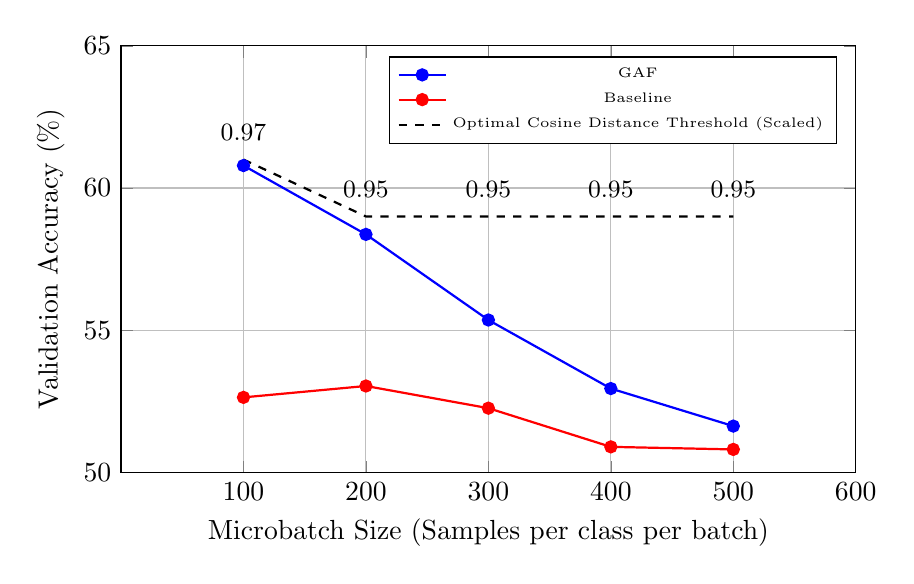
\begin{tikzpicture}
        \begin{axis}[
            % title={Microbatch Size on Validation Accuracy on CIFAR-100N-Fine},
            xlabel={Microbatch Size (Samples per class per batch)},
            ylabel={Validation Accuracy (\%)},
            xmin=0, xmax=600,
            ymin=50, ymax=65,
            xtick={100, 200, 300, 400, 500, 600},
            ytick={50, 55, 60, 65},
            legend style={at={(0.975,0.975)}, anchor=north east, font=\tiny},
            grid=both,
            width=0.9\columnwidth,
            height=7cm,
        ]

        % Plot GAF Validation Accuracy
        \addplot[
            color=blue,
            mark=*,
            thick,
        ] coordinates {
            (100, 60.79)
            (200, 58.37)
            (300, 55.36)
            (400, 52.95)
            (500, 51.63)
        };
        \addlegendentry{GAF}

        % Plot Baseline Validation Accuracy
        \addplot[
            color=red,
            mark=*,
            thick,
        ] coordinates {
            (100, 52.64)
            (200, 53.04)
            (300, 52.26)
            (400, 50.90)
            (500, 50.81)
        };
        \addlegendentry{Baseline}

        % Plot Optimal Cosine Distance Threshold with custom labels
        \addplot[
            color=black,
            dashed,
            mark=none,
            thick,
            nodes near coords={
                \pgfmathparse{\coordindex == 0 ? "0.97" : "0.95"} \pgfmathresult
            },
            every node near coord/.append style={font=\small, anchor=south, yshift=3pt}
        ] coordinates {
            (100, 61) % Approximated y-values to fit within the y-axis range
            (200, 59)
            (300, 59)
            (400, 59)
            (500, 59)
        };
        \addlegendentry{Optimal Cosine Distance Threshold (Scaled)}

        \end{axis}
    \end{tikzpicture}
    
    \caption{ResNet34 PreAct Validation accuracy over microbatch size in the GAF and baseline case on CIFAR-100N-Fine, overlaid with cosine distance threshold used in training. As we increase microbatch size, the benefit of GAF reduces due to averaging more noisy samples.}
    \label{fig:cifarn-microbatch-size}
\end{figure}

% \subsubsection{ImageNet}

% For all ILSVRC12 runs we use ViT-L/16. We train with microbatch size of 380 and a macro batch size of 2. We train on 2xH100s. We use AdamW with a linear warmup of 100 iters and Cosine LR schedule with num cycles = 5 and learning rate 3e-5. We use weight decay of 0.05 and betas of (0.9, and 0.999). As we can not fit one image per class as their are 1000 classes we sample 380 classes of the 1000 and sample 2 images per class and send one to each of the GPU ranks to process so the mini batches are completely iid. We vary cosine distance threshold from 0.95-1.05 with a step of 0.01. We also use cosine distance threshold of 2 for the baseline runs. 

% \subsection{Toy Experiments}
% Omitted for now not working
% \textbf{TODO}: Duncan to fill in.
